
\chapter{Definición formal del problema}

Tanto el problema que planteamos abordar como la solución propuesta son complejos de definir, ya que incluye numerosos conceptos del procesamiento de lenguaje natural. En la primera parte de esta sección definiremos un marco teórico para cada aspecto no central del problema. A partir de esta base, en la segunda parte daremos una definición propiamente dicha, seguida por una formalización de la solución.

\section{Datos Enlazados y Sistemas de Respuesta}

La cantidad de infomación disponible en internet es abrumadora, y sin embargo, aún no puede utilizarse en conjunto para extracción de infomación satisfactoriamente. \citet{BernersLeeLinkedDataGuide} explican que este fenómeno se debe a que fragmentos de información que se refieren al mismo objeto o suceso no están relacionados entre sí

\citet{BizerLinkedData} definen los datos enlazados como infomación que cumple las siguientes características:
\begin{enumerate}
    \item Puede ser leída automáticamente por una computadora.
    \item Su significado está explícitamente definido.
    \item Está conectada a fuentes de datos externas.
    \item Puede ser conectada desde fuentes de datos externas a su vez.
\end{enumerate}
% Berners-Lee, T. (2006). Linked Data - Design Issues. Retrieved July 23, http://www.w3.org/DesignIssues/LinkedData.html
% Cómo cito cosas que saco de internet y que no están en una publicación?
Sin embargo, no existe un conceso o una definición formal sobre el tema. \citet{BernersLeeLinkedDataGuide} describe en su artículo un protocolo orientativo para publicar datos enlazados en la web de tal forma que pudiera formase una base de conocimiento global. Con el tiempo estas reglas se han tomado como un estándar para la construcción de ontologías, y en la actualidad existen espacios de información que contienen millardos de aserciones del mundo real.

% Brickley, D., Guha, R. (2004). RDF Vocabulary Description Language 1.0: RDF Schema - W3C Recommendation. Retrieved June 14, 2009, http://www.w3.org/TR/rdf-schema/
Los datos enlazados se representan comunmente como una colección de tripletas siguiendo un lenguaje de descripción como RDF, tal como lo describe \citet{brickleyRDF}. Cada tripleta se compone de un sujeto, un predicado y un objeto, donde el predicado representa una relación entre el sujeto y el objeto. De esta forma se puede representar cualquier tipo de asociación entre entidades sin importar su complejidad, contruyéndolo a partir de relaciones parciales. El resultado es información organizada en forma de grafo donde cada nodo es una entidad y cada arista es una relación entre dichas entidades.

Las web semánticas u ontologías más populares en el momento son FreeBase \footnote{www.freebase.com} y DBPedia \footnote{www.dbpedia.org}, aunque existen numerosos proyectos con dominios más acotados como WordNet \footnote{www.wordnet.princeton.edu}. Estas plataformas son abiertas con interfaces fáciles de utilizar que permiten agregar nuevos datos, y como resultado se observa un rápido crecimiento en la cantidad de información disponible.

Estos sitios cuentan con puertos de accesos donde los usuarios pueden enviar consultas utilizando algún lenguaje formal. Aunque este servicio es accesible para cualquier persona, se requiere cierto nivel de conocimiento técnico para generar dichas consultas. Para dar acceso real a las masas a esta gran cantidad de información de requieren interfaces capaces de extraer datos a partir de consultas en lenguaje natural, es decir, sistemas de respuestas a preguntas.

Paralelamente, los sistemas de respuesta a preguntas pueden obtener grandes beneficios de una ontología. En lugar de buscar documentos o pasajes que puedan contener una respuesta, los datos enlazados pueden brindar información exacta. Además de ello, resulta más fácil procesar preguntas donde es muy poco probable encontrar la respuesta en un solo documento, por ejemplo, ``¿Qué famosas actrices nacieron en el mismo país que Naima Akef?''. Desde los años 70 este tipo de software ha utilizado bancos de conocimiento estructurada que inicialmente eran bases de datos locales. Sin embargo, los resultados obtenidos no se destacaron particularmente. Con el desarrollo de las nuevas web semánticas la atención ha vuelto nuevamente hacia los datos relacionados.

Extraer información de una ontología no es difícil, sin embargo, como describe \citet{ungerQALD}, indentificar el sector de datos relevante a una consulta en lenguaje natural es un gran desafío. Se requiere para esto traducir el texto ingresado por el usuario en una consulta formal que pueda ser procesada por un motor de búsqueda tradicional sobre datos enlazados. Una vez que se ha obtenido la información de la base, otra etapa de procesamiento convierte estos datos del formato legible por una computadora a un formato legible por el usuario. A continuación ilustramos con un ejemplo estas etapas utilizando una consulta en lenguaje MQL sobre la estructura de FreeBase.

\begin{example}\label{QALD-etapas}\hfill
    \begin{enumerate}
        \item Obtención de la pregunta.
            \begin{lstlisting}
    What is the capital city of Argentina?
            \end{lstlisting}
        \item Generación de la consulta MQL.
            \begin{lstlisting}
    {
        "type":"/location/country",
        "id":"/en/argentina",
        "capital":null
    }
            \end{lstlisting}
        \item Obtención de la información.
            \begin{lstlisting}
    {
        "result": {
            "capital": "Buenos Aires",
            "type": "/location/country",
            "id": "/en/argentina"
        }
    }
            \end{lstlisting}
        \item Generación de la respuesta en leguaje natural.
            \begin{lstlisting}
    The capital city of Argentina is Buenos Aires.
            \end{lstlisting}
    \end{enumerate}
\end{example}

El primer desafío es identificar la entidad a la que se hace referencia en la pregunta, en nuestro caso, ``Argentina''. Esta tarea se complicaría con nombre más complejos como ``People's Republic of China''. Las complicaciones de este etilo está ligadas a los sistemas externos de parseo y asignación de etiquetas morfosintácticas. Sin un buen procesamiento del lenguaje natural poco puede contruirse.

Adicionalmente, las consultas contienen no sólo información brindada por la pregunta del usuario, sino también datos asociados a la estructura de la base. Si en lugar de ``/location/country'' hubieramos utilizado ``/location/location'' la consulta hubiera devuelto un error, a pesar de que Argentina es también de tipo ``/location/location''. \citet{ungerQALD} menciona también otros problemas que frecuentemente enfrentan este tipo de sistemas.

En las consultas utilizando MQL se detalla la estuctura de la información y se completan los datos necesarios para identificar el objeto en la base de datos. Para obtener información sobre la entidad se nombran sus atributos, pero se les da un valor de $null$. El motor de búsqueda identifica estos campos y completa la información faltante. Este lenguaje es muy intuitivo y fue diseñado para ser accesible, pero no todos los lenguajes de consulta son tan simples como MQL.

\vspace{5mm}
\begin{example} Consulta en SPARQL para la pregunta ``How many episodes does Seinfeld have?''
    \begin{lstlisting}
    PREFIX rdf: <http://www.w3.org/1999/02/22-rdf-syntax-ns#>
    PREFIX dbpprop: <http://dbpedia.org/property/>
    PREFIX dbpedia-owl: <http://dbpedia.org/ontology/>

    SELECT DISTINCT ?x1 WHERE {
      ?x0   rdf:type                        dbpedia-owl:TelevisionShow.
      ?x0   dbpprop:showName                "Seinfeld"@en.
      ?x0   dbpedia-owl:numberOfEpisodes    ?x1.
    }
    \end{lstlisting}
\end{example}

La cantidad de información necesaria para construir esta consulta es mucho mayor mientras que su estructura no es simple de comprender. Sin embargo, pone en relevancia el uso de tripletas para representar la relación entre distintos nodos. En particular, la variable $?x1$ representa el resultado, mientras que la variable $?x0$ representa a la entidad de nombre ``Seinfield'' y tipo ``TelevisionShow''.

Cómo cierro esta sección? Quiero dar una buena introducción a las consultas para después explicar bien cómo funciona Quepy.


\section{Quepy}

Como se mencionó anteriormente, Quepy es un marco de trabajo para crear aplicaciones de respuesta a preguntas. Su objetivo principal es brindar una herramienta fácilmente adaptable a distintos dominios y distintos lenguajes de consultas. Los lenguajes soportados hasta el momento son MQL y SPARQL; ambos permiten consultas posteriores a FreeBase y DBPedia. Haremos un breve resumen a continuación sobre la arquitectura general de Quepy y sus principales características.

Una aplicación creada en Quepy tiene tres secciones principales:
\begin{description}
    \item[Settings] La configuración de Quepy incluye las herramientas de análisis sintáctico a utilizar, la URL del servidor para enviar las consultas, etc.
    \item[Templates] Contiene las plantillas definidas por el creador de la aplicación. Cada plantilla es una expresión regular que combina distintos tipos de caracteríticas como etiquetas POS y lemmas, lo que permite al sistema identificar la semántica de la pregunta únicamente en base a su sintáxis. Junto con la expresión regular, cada plantilla tiene una función de interpretación que toma las secciones de la pregunta que considera relevantes y las utiliza para construir una representación interna de la pregunta llamada Expresión.
    \item[DSL] Son las siglas correspondientes a Lenguaje de Dominio Específico en inglés. En esta selección se detalla cómo las Expresiones de Quepy se traducen a las partes integrantes de una consulta formal.
\end{description}

A grandes rasgos, Quepy utiliza dos etapas que traducen una pregunta a una Expresión y luego utilizan la Expresión para formar consultas. Esto es así ya que permite soportar diversos lenguajes de consultas. Estas representaciones internas son generales y pueden generar cualquier consulta. Es el programador quien se encarga de especificar las reglas de construcción de las expresiones y las de traducción a lenguaje formal, por ejemplo SPARQL.

\subsection{Construcción de las consultas}

Para entender mejor cómo funciona Quepy internamente veamos en ejemplo en particular, extraído de la documentación oficial \footnote{http://quepy.readthedocs.org/en/latest/tutorial.html}. Este ejemplo corresponde a una aplicación realizada para generar consultas SPARQL para ser enviadas a un motor de la DBPedia. Analicemos primero cómo se definen los elementos del DSL para luego seguir con las plantilla propiamente dichas.

\begin{example}Definición de un elemento del DSL.
    \begin{lstlisting}
    from quepy.dsl import FixedRelation

    class IsDefinedIn(FixedRelation):
        relation = "rdfs:comment"
        reverse = True
    \end{lstlisting}
\end{example}

La clase $IsDefinedIn$ es una Expresión que representa una relación entre dos objetos, como vimos anteriormente en RDF. Dependiendo del lenguaje de consulta tendrá distinas traducciones, y en particular para SPARQL es equivalente a:

\begin{lstlisting}
?target rdfs:comment ?definition
\end{lstlisting}

donde $?target$ y $?definition$ son parámetros que tomará la Expresión al instanciarse.

Las expresiones pueden construirse progresivamente a partir de otras expresiones como veremos a continuación.

\begin{example}\label{plantilla-quepy} Plantilla para las preguntas de tipo ``What is ... ?''.
    \begin{lstlisting}
    from refo import Group, Question
    from quepy.dsl import HasKeyword
    from quepy.parsing import Lemma, Pos, QuestionTemplate

    from dsl import IsDefinedIn

    class WhatIs(QuestionTemplate):

        aux = Question(Pos("DT")) + Group(Pos("NN"), "target")
        regex = Lemma("what") + Lemma("be") + aux + Question(Pos("."))

        def interpret(self, match):
            thing = match.target.tokens
            target = HasKeyword(thing)
            definition = IsDefinedIn(target)
            return definition
    \end{lstlisting}
\end{example}

Observemos que la clase tiene un attributo llamado $regex$ que corresponde a la expresión regular que define la plantilla. Profundizaremos en la estructura de estas expresiones regulares más adelante, pero ahora notemos que uno de los elementos tiene una etiqueta $target$. Si la pregunta ingresada por el usuario concuerda con esta expresión regular, entonces los elementos que concuerden con las sub expresiones etiquetadas serán pasados al método $interpret$ de la clase. En este caso, el segmento de oración que corresponda a $Group(Pos("NN"))$ (un conjunto de sustantivos) será un atributo del parámetro $match$ recibido por $interpret$.

El método $interpret$ construye una Expresión de tipo $HasKeyword$ a partir de $target$ y luego la utiliza para contruir otra Expresión de tipo $IsDefinedIn$. El resultado final de la Expresión traducida a SPARQL para la pregunta ``What is a car?'' será:

\vspace{5mm}

\begin{lstlisting}
PREFIX rdfs: <http://www.w3.org/2000/01/rdf-schema#>
PREFIX quepy: <http://www.machinalis.com/quepy#>

SELECT DISTINCT ?x1 WHERE {
  ?x0 quepy:Keyword "car".
  ?x0 rdfs:comment ?x1.
}
\end{lstlisting}

\vspace{5mm}

\subsection{Plantillas y sus expresiones regulares}

Describiremos a continuación más en detalle la estructura de las plantillas que permiten crear una Expresión a partir de una pregunta. Cada una de las plantillas está construida en base a la librería REfO\footnote{https://github.com/machinalis/refo}, que define expresiones regulares entre objetos complejos de Python, no solamente cadenas de caracteres.

\begin{example}\label{regex} Expresión regular del ejemplo \ref{plantilla-quepy}\footnote{Reemplazamos la variable aux por su contenido para mayor claridad, lo cual no afecta el significado de la expresión regular.}.
    \begin{lstlisting}
    regex = Lemma("what") + Lemma("be") + Question(Pos("DT"))
            + Group(Pos("NN"), "target") + Question(Pos("."))
    \end{lstlisting}
\end{example}

Para analizar si un frase concuerda o no con una expresión regular, Quepy transformará la oración con el analizador sintáctico indicado para obtener el lemma y las etiqueta POS de cada una de sus palabras. Luego, utilizará esa información para compararla con la expresión regular. Entonces, nuestro ejemplo concordará con una frase cuya primera palabra tenga lemma ``what'', su segunda palabra tenga lemma ``be'', su tercera palabra (opcionalmente) tenga etiqueta POS ``DT'', etc.

Dada una pregunta, Quepy intentará encontrar una concordancia con cada una de estas expresioner regulares existentes. Si la encuentra, entonces utilizará el método $interpret$ que explicamos en la sección anterior para construir una Expresión y luego una consulta.

Definir patrones de reconocimiento de esta manera permite representar tanto información semántica como sintáctica y por lo tanto tienen mayor poder expresivo que cualquiera de ellas por separado. Veremos más adelante que elegimos estos patrones como una forma de representación de las preguntas para clasificar.

\section{Formalización del problema}

A pesar de las numerosas ventajas de Quepy, también existen desventajas. La más importante de ellas es que, al utilizar expresiones regulares, los patrones no tienen flexibilidad y dependen fuertemente del analizador sintáctico y POS tagger que utilicen.

En particular, si tomamos el ejemplo de la sección anterior, no se podrían reconocer preguntas del estilo ``Definition of a car'' o ``How would you define what a car is?''. La respuesta a estas preguntas se obtiene con la misma consulta generada que acabamos de analizar, por lo cual son escencialmente equivalentes. Diremos entonces que estas preguntas comparten la misma semántica, y que son reformulaciones una de la otra.

Para agregar un nuevo tipo de pregunta al sistema se deben definir sus patrones y sus traducción a una consulta. Gracias a la gran cantidad de formas distintas en las que se puede expresar una pregunta es imposible construir todas las expresiones regulares necesarias, y los sistemas de Quepy están fuertemente limitados por esta característica. Si los patrones fueran más generales o pudieran inferirse de alguna forma, entonces ampliar los tipos soportados consistiría sólo en el segundo paso.

\citet{ungerQALD} clasifica los sistema de respuesta a preguntas sobre datos enalzados (QALD por sus siglas en inglés) según sus estrategias de resolución de la pregunta. Entre ellos se encuentra la clase a la cual pertenece Quepy, llamada por los autores ``Template-Based approaches'' o Aproximaciones Basadas en Patrones. Claramente, la falta de cobertura sobre el universo posible de preguntas en una dolencia de cualquier sistema que utilice patrones estáticos para clasificar las preguntas en una determinada representación.

Lo que nos proponemos entonces lograr con este trabajo es ampliar la cobertura de un sistema QALD basado en concordancia con patrones para reconocer preguntas semánticamente equivalentes a una de sus clases ya definidas en él. El sistema QALD que tomamos como base es Quepy, en particular una aplicación realizada como demostración del producto\footnote{Puede utilizarse online ingresando a http://quepy.machinalis.com/}. A partir de este punto, utilizaremos la palabra Quepy para referirnos tanto al marco de trabajo como a las aplicaciones construidas por él, y en particular a la que estaremos usando.

\section{Solución propuesta}

Como la generación de nuevas plantillas manualmente no es viable, entonces proponemos una solución automática: agregar al sistema un clasificador que identifique (si existiera) el patrón que corresponde a la pregunta. Es tarea del clasificador asociar reformulaciones que tengan la misma semántica a solo patrón. Una vez obtenida la clase semántica e identificado el objeto de la pregunta, Quepy u otro sistema puede construir la consulta directamente. Dejaremos como trabajo futuro el reconocimiento de la entidad base y nos centraremos en la clasificación de las preguntas.

Este enfoque de encontrar reformulaciones de una misma pregunta está enmarcado dentro del reconocimiento de implicaciones textuales y ha sido utilizado previamente para sistema de respuesta a preguntas del usuario. \citet{ou_entailement} utilizan esta técnica tomando como base preguntas modelo construidas automáticamente desde la ontología, y se centran también en la composición de patrones simples para formar otros más complejos. Sin embargo, se limitan a un dominio muy restringido que permite formar texto en lenguaje natural desde las relaciones formales entre las entidades, lo cual sería dificultoso en ontologías complejas como FreeBase. \citet{rui_relations} explican otros posibles usos de identificar estas relaciones entre las preguntas para sugerencia de preguntas relacionadas o útiles para el usuario. El trabajo de \citet{Kosseimmuyparecido}, por otra parte, utiliza la reformulación para obtener patrones semánticamente equivalente, pero utiliza durante el entrenamiento del clasificador la respuesta de la pregunta.

Nuestro trabajo será construir y entrenar un clasificador capaz de recibir una pregunta y decidir a qué clase semántica pertenece, siguiendo la definición de \citet{Sebastiani-text-categorization}:

\begin{definition}
La clasificación de una instancia es una función $\Psi:\mathcal{X} \times \mathcal{C} \rightarrow \{0, 1\}$ que asigna valores booleanos donde $\mathcal{X}$ es el dominio de las instancias y $\mathcal{C}$ es el conjunto de clases posibles.
\end{definition}

Asignaremos el valor $1$ o $Verdadero$ a los pares $\langle x_i, c_j \rangle$ si la clase $c_j$ corresponde a la instancia $x_i$, y $0$ o $Falso$ en el caso contrario. Como en nuestro caso la clase asociada a cada instancia es única, podemos utilizar la siguiente definición:

\begin{definition}\label{def-clasificacion}
Un clasificador monoclase es una función $\Phi:\mathcal{X} \rightarrow \mathcal{C}$ tal que:
$$ \Phi(x_i) = c_j \Leftrightarrow \Psi(x_i, c_j) = 1 $$
\end{definition}

$\mathcal{C}$ para esta clasificación es el conjunto de clases semánticas de Quepy, es decir, cada una de las plantillas o patrones. El ejemplo que describimos en la sección anterior corresponde a la clase ``Whatis''. Todas las preguntas que puedan responderse a través de la consulta generada por esta plantilla serán clasificadas dentro de esta clase. La cantidad total de clases es 29, las agregamos en un APENDICE?



%Pocas preguntas como semillas, muchas preguntas no etiquetadas => aprendizaje activo
% Cómo representar la clase semántica de una pregunta => características usadas y aprendizaje sobre características.

Aunque la tarea a realizar no parece compleja y ha sido ampliamente estudiada, nos encontramos con numerosos obstáculos que impiden utilizar algún método estándar de clasificación de texto. A continuación discutiremos dos de estos incovenientes y las decisiones que tomamos para resolverlos.

\subsection{De la Clasificación Supervisada al Aprendizaje Activo}

En primer lugar, no contamos con un corpus anotado que permita utilizar clasificación supervisada común. Desarrollamos entonces un pequeño corpus a partir de los ejemplos incuidos en Quepy. Por cada clase agregamos también algunos casos de reformulaciones no reconocidos por la aplicación y también las etiquetamos. El resultados final fueron 106 preguntas, un número más que modesto y que difícilmente cubre el universo de posibles reformulaciones de todas las clases.

Sin embargo, existen numerosos corpus de preguntas utilizados para otras tareas de clasificación que no están etiquetados. Por lo tanto, decidimos utilizar un enfoque semiautomático que comience con un conjunto de semillas y que utilice las preguntas no etiquetadas paulatinamente para aprender la clasificación. Esto nos permitirá compensar la falta de cobertura sobre el dominio.

La fuente más importante de preguntas para la construcción del corpus no anotado fueron las preguntas de entrenamiento y evaluación de las tareas del TREC\footnote{http://trec.nist.gov/data/qamain.html} desde el año 2008. Por lo tanto, consideramos que nuestro conjunto representativo de las posibles preguntas que un usuario podría esperar que un sistema responda. Sin embargo sólo una porción muy pequeña del ellas se corresponde con alguna de las clases de Quepy. Por lo tanto, entrenar un casificador con tan alta cantidad de ruido sería una tarea muy difícil.

Tengamos en cuenta también que los límites de una clase semántica no siempre están claros y algunas veces dependen fuertemente de la estructura de los datos en la ontología.

\begin{example}\label{preguntas-similares}\hfill
    \begin{enumerate}
    \item ``What is the tallest mountain?''
    \item ``What is the Everest mountain?''
    \end{enumerate}
\end{example}

Estas preguntas son muy similares, y sin embargo sólo la segunda pertenece a la case ``whatis'': para responder la primera pregunta debe obtenerse la altura de todas las montañas de la base de datos y seleccionar la mayor.

Por este motivo decidimos utilizar una plataforma de aprendizaje activo donde un oráculo humano ayudará al sistema a delimitar estas sutilezas semánticas. \citet{rare-classes-holpedales} y \citet{AL-imbalanced-Ertekin} describe clasificadores adaptados a través del aprendizaje activo para encontrar y clasificar ejemplos raros de clases minoritarias. Además de ello, el aprendizaje activo es una estrategia que obtiene buenos resultados para problemas con una gran cantidad de clases, de acuerdo con \citet{al-multiclass-jain}.

\citet{settles_active_learning_survey} explica que el aprendizaje activo es un paradigma donde el aprendedor selecciona preguntas para que un humano u oráculo las etiquete. Si el aprendedor elige las instancias de las cuales puede aprender más información, entonces se minimiza la cantidad de instancias etiquetadas necesarias para lograr el mismo desempeño. La mayor motivación para este tipo de estrategias es la dificultad de conseguir dato etiquetados al mismo tiempo que se disponen de grandes cantidad de ejemplos no etiquetados, tal y como es nuestro caso. Utilizaremos aprendizaje activo para conseguir un corpus etiquetado de entrenamiento con el menor esfuerzo posible.

\begin{figure}[h]
\caption{Arquitectura de un sistema de aprendizaje activo}
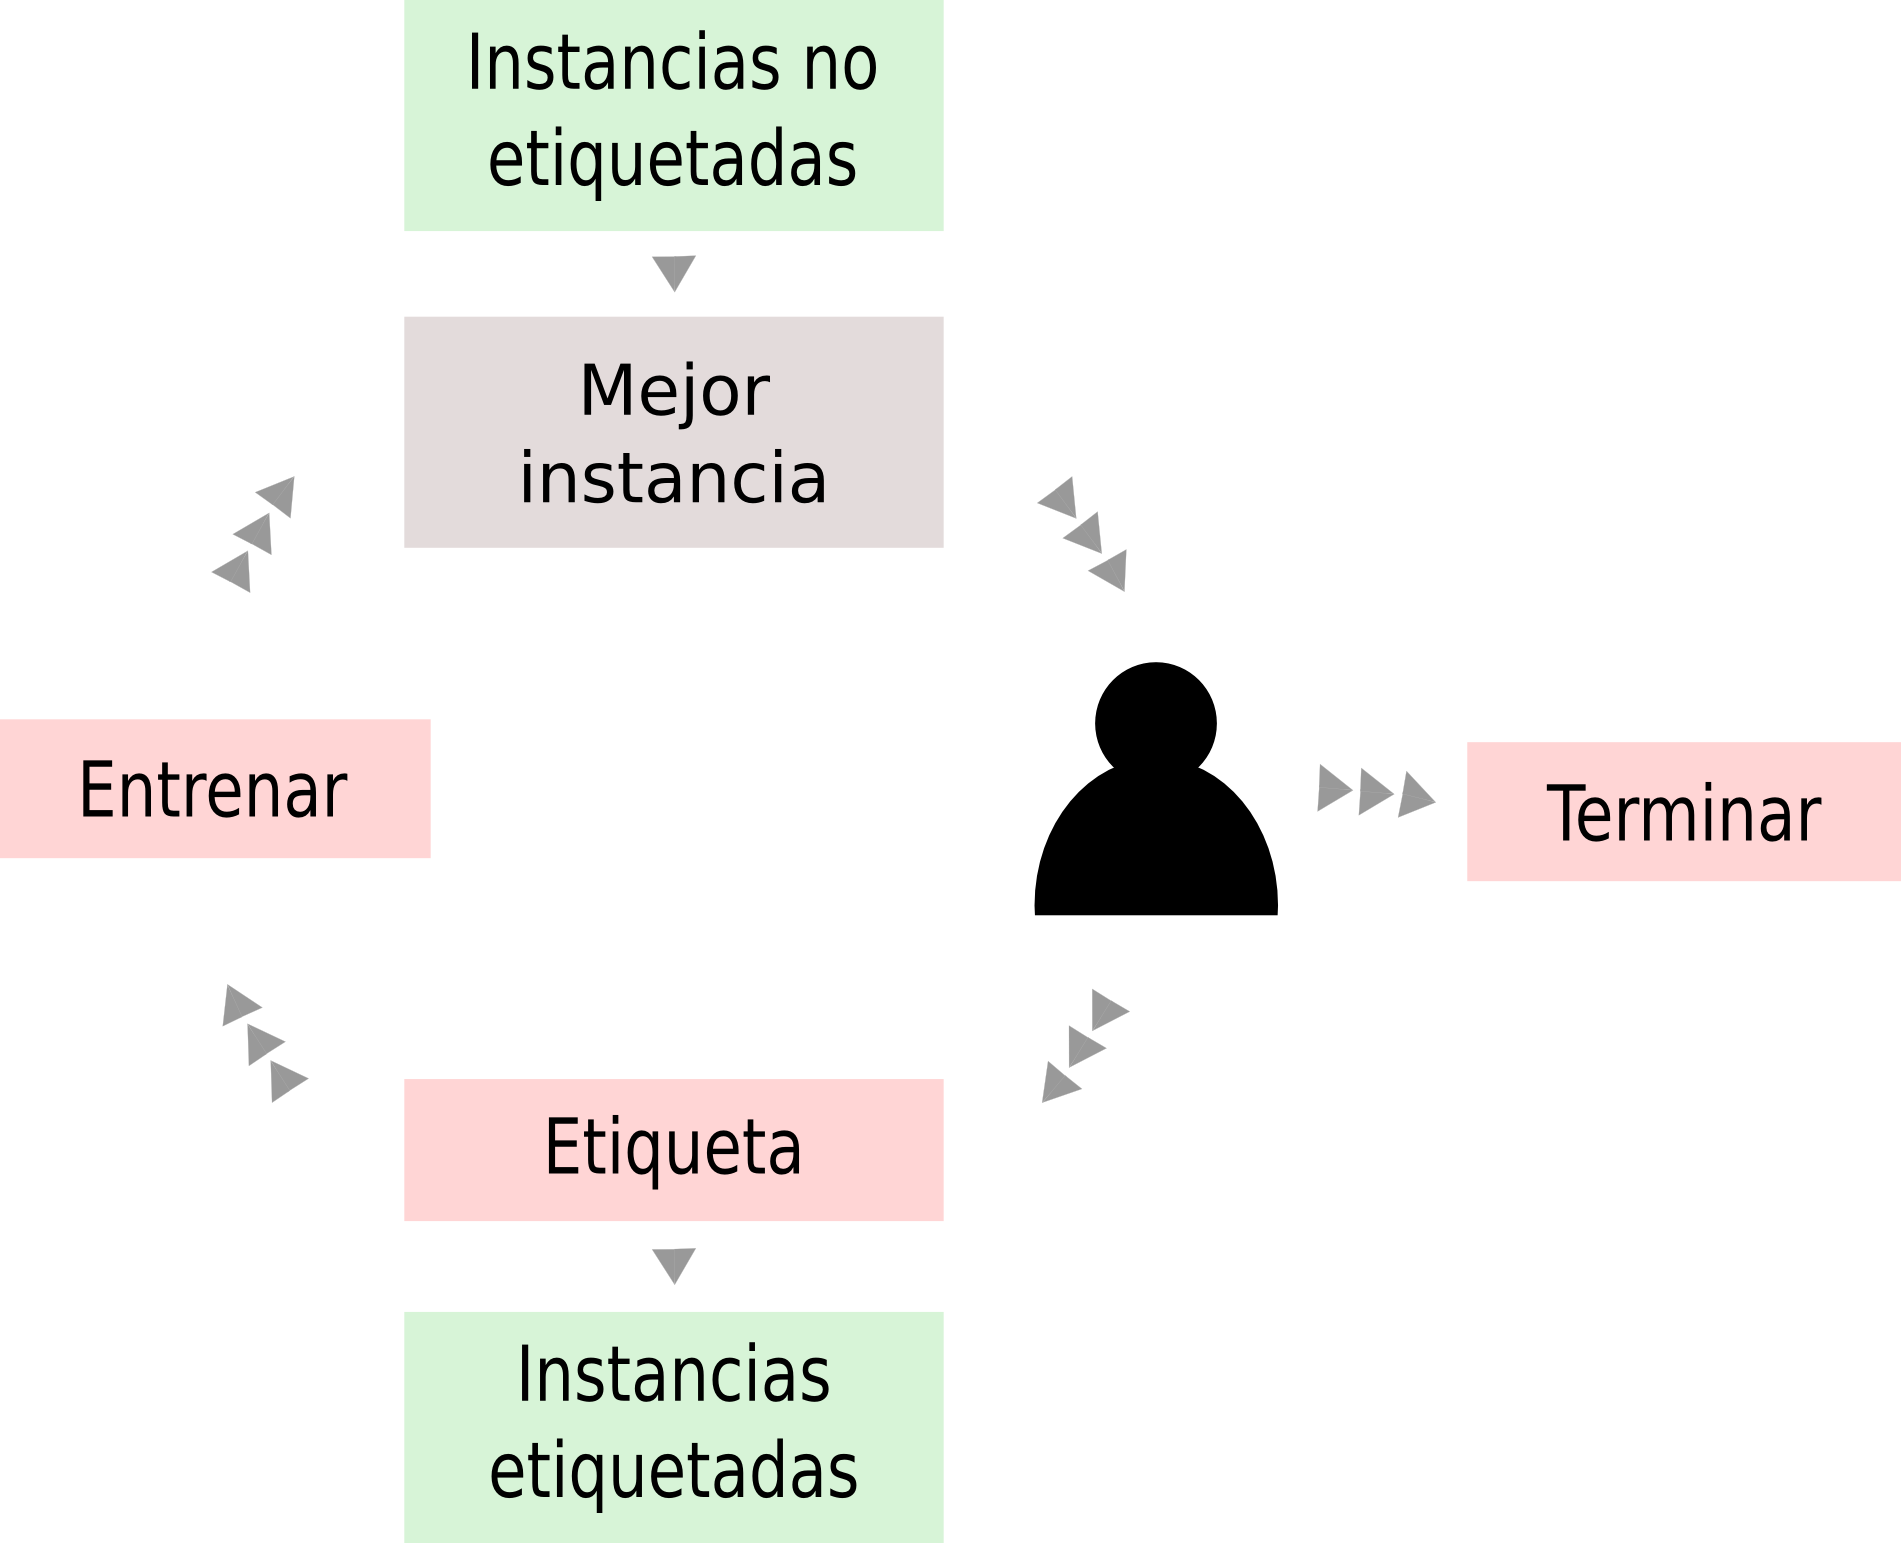
\includegraphics[width=8cm]{cicloaa.png}
\centering
\end{figure}

\subsection{Aprendizaje activo sobre características}

Durante las primeras etapas de desarrollo y especificación del problema debimos definir la representación de las instancias ante el clasificador. Sin embargo, al no existir trabajos previos con la misma proximación al problema no tenemos un punto de referencia para tomar como ejemplo. Por esto, decidimos incluir características tentativamente y realizar experimentos con aprendizaje activos sobre características e instancias.

%nos ayuda a entender mejor

En un enfoque como este se pedirá al usuario que etiquete las características seleccionadas con una clase si la presencia de la característica en una instancia es indicativa de la clase. \citet{settles-al-features} han realizado experimentos sobre clasificación de texto en donde se demuestra que el aprendizaje activo sobre características puede dar mejores resultados incluso que el aprendijase sobre instancias. Durante este trabajo ayudará a identificar las características que mejor describen las instancias para la clasificación descripta.

Las etiquetas obtenidas se utilizarán también para entrenar el clasificador reforzando la probabilidad de una característica dada una clase, como veremos en detalle en la implementación.

\subsection{Dualist}

Dualist es un sistema muy similar al que estamos planteando desarrollado por \citet{dualist} que combina el aprendizaje sobre instancias y sobre características. Los resultados presentados son para diversas tareas como el análisis de sentimientos o la clasificación de documentos.

La interfaz gráfica de una instancia tiene dos secciones principales. A la izquierda se muestra una lista de instancias con las clases para que el usuario pueda etiquetarlas sólo con un click. A la derecha, por cada clase hay una lista de objetos seleccionables representando las características (en este caso palabras) que están potencialmente asociadas a la clase. \citet{dualist} sostienen que presentar al usuario toda la información en conjunto hará que éste etiquete una mayor cantidad antes de esperar a que el clasificador de reentrene o le presente nuevas opciones.

\begin{figure}
\caption{Captura de pantalla de la interfáz gráfica de Dualist.}
\includegraphics[width=12cm]{dualist-screen}
\centering
\end{figure}

Nuestra implementación seguirá los mismos lineamientos principales y pondremos en práctica las técnicas de selección de ejemplos con las de entrenamiento del clasificador para obtener resultados sobre nuestra configuración. Decidimos tomarlo como modelo ya que se centra en la interacción con el usuario y en la capacidad del software de ser utilizado en tiempo real. Nosotros deseamos lograr un sistema que sea viable de integrar con Quepy y complementar aplicaciones reales, en lugar de ser utilizado sólo para demostrar los resultados de este trabajo.

